\documentclass[10pt]{article}
\usepackage{graphicx}
\usepackage{amssymb}
\usepackage[fleqn]{amsmath}
\usepackage{nccmath}
\usepackage{cases}
\usepackage{hyperref}
\usepackage{multicol}
\usepackage{tikz}
\usepackage{pgfplots}
\usepackage{enumitem}
\usepackage{pdfpages}
\pgfplotsset{compat=1.18}
\usepackage{float}


\title{\bf Math 151b: Problem Set 6}
\date{2/23/2024}
\author{\bf Owen Jones}
\begin{document}
\maketitle

\noindent\textbf{Problem 1}\\
Suppose a solution $u(x)$ exists.\\
We use the  divergence theorem:
$\displaystyle \int_{a}^{b}u''(x)dx=u'(b)-u'(a)$.\\
We are given $u''(x)=f(x)$, $u'(a)=\alpha$, and $u'(b)=\beta$.
Substituting into our equation, we obtain $\displaystyle \int_{a}^{b}f(x)dx=\beta-\alpha$.\\
The solution to the Neumann problem is not unique because it does not take into account the absolute temperature of the bar. 
$u(x)$ and $u(x)+c$ can both be solutions to the problem, but one solution can have a higher absolute temperature at every point on the interval.\\
\textbf{Problem 2}\\
$u(x_{j+1})=u(x_j+h)=u(x_j)+hu'(x_j)+\frac{h^2}{2}u''(x_j)+\frac{h^3}{6}u'''(x_j)+O(h^4)\\
u(x_{j-1})=u(x_j-h)=u(x_j)-hu'(x_j)+\frac{h^2}{2}u''(x_j)-\frac{h^3}{6}u'''(x_j)+O(h^4)$\\
The zeroth, first, and third derivatives cancel out leaving\\
$\frac{u(x_{j+1})-2u(x_j)+u(x_{j-1})}{h^2}=\frac{h^2u''(x_j)+O(h^4)}{h^2}=u''(x_j)+O(h^2)$.\\
\textbf{Problem 3}\begin{enumerate}[label=(\alph*)]
    \item Because $\mathbf{x}$ is a vector s.t $A\mathbf{x}=\mathbf{0}$ $\displaystyle \sum_{j=1}^{n}a_{ij}x_j=0$ $\forall i=1\ldots n$.
    Fix some $i$. It follows $\displaystyle a_{ii}x_i=-\sum_{j=1,j\neq i}^{n}a_{ij}x_j$. 
    Taking the absolute value of both sides, we obtain $\displaystyle\lvert a_{ii}\rvert \lvert x_i\rvert=\lvert a_{ii}x_i\rvert=\lvert -\sum_{j=1,j\neq i}^{n}a_{ij}x_j\rvert=\lvert\sum_{j=1,j\neq i}^{n}a_{ij}x_j\rvert$.\\
    Thus, $\displaystyle\lvert a_{ii}\rvert \lvert x_i\rvert=\lvert\sum_{j=1,j\neq i}^{n}a_{ij}x_j\rvert$.
    \item Applying the Triangle Innequality to the RHS of (2), we obtain \\
    $\displaystyle\lvert\sum_{j=1,j\neq i}^{n}a_{ij}x_j\rvert\le\sum_{j=1,j\neq i}^{n}\lvert a_{ij}\rvert \lvert x_j\rvert$.\\
    Using (3) i.e $\lvert x_i\rvert =\max\underset{1\le j\le n}{\lvert x_j\rvert}$, we obtain\\
    $\displaystyle \sum_{j=1,j\neq i}^{n}\lvert a_{ij}\rvert \lvert x_j\rvert\le \sum_{j=1,j\neq i}^{n}\lvert a_{ij}\rvert \lvert x_i\rvert$.\\
    Together with (1) $\displaystyle \sum_{j=1,j\neq i}^{n}\lvert a_{ij}\rvert < \lvert a_{ii}\rvert$ we obtain\\
    $\displaystyle \lvert\sum_{j=1,j\neq i}^{n}a_{ij}x_j\rvert\le\sum_{j=1,j\neq i}^{n}\lvert a_{ij}\rvert \lvert x_i\rvert< \lvert a_{ii}\rvert\lvert x_i\rvert$\\
    which is a contradiction because we claimed $\displaystyle \lvert\sum_{j=1,j\neq i}^{n}a_{ij}x_j\rvert=\lvert a_{ii}\rvert\lvert x_i\rvert$.\\
    Thus, $A$ must be non-singular.
\end{enumerate}
\textbf{Problem 4}\\
\begin{enumerate}[label=(\alph*)]
    \item The central difference formula for $u''(x_i)\approx\frac{u(x_{i+1}-2u(x_i)+u(x_{i-1}))}{h^2}$.\\
    Thus, $f(x_i)=\frac{u(x_{i+1}-2u(x_i)+u(x_{i-1}))}{h^2}-cu(x_i)=\frac{u(x_{i+1}-(2+ch^2)u(x_i)+u(x_{i-1}))}{h^2}$.\\
    Let $\mathbf{u}={[u_1,u_2,\ldots,u_{N-1}]}^\top$ and $\mathbf{f}={[f_1,f_2,\ldots,f_{N-1}]}^\top$ where $u_i=u(x_i)$ and $f_i=f(x_i)$.\\
    \item At the boundaries we have $\frac{\alpha-(2+ch^2)u_1+u_2}{h^2}=f_1\Rightarrow \frac{-(2+ch^2)u_1+u_2}{h^2}=f_1-\frac{\alpha}{h^2}$ and $\frac{u_{N-2}-(2+ch^2)u_{N-1}+\beta}{h^2}=f_{N-1}\Rightarrow \frac{u_{N-2}-(2+ch^2)u_{N-1}}{h^2}=f_{N-1}-\frac{\beta}{h^2}$.\\
    Thus, our matrix $A:(N-1)\times (N-1)$ can be represented as\\ 
    $A=\frac{1}{h^2}\begin{bmatrix}
        -(2+ch^2) & 1 & 0 & 0 & \cdots & 0\\
        1 & -(2+ch^2) & 1 & 0 & \cdots & 0\\
        0 & \ddots & \ddots & \ddots & \ddots & 0\\
        \cdots & \cdots & \cdots & \cdots & \cdots & \cdots\\
        0 & \cdots & 0 & 0 & 1 & -(2+ch^2)
    \end{bmatrix}$\\
    giving us $A\mathbf{u}=\mathbf{f}-{[\frac{\alpha}{h^2},0,\ldots,0,\frac{\beta}{h^2}]}^\top$\\
    Fix some row $i$.\\ 
    $\displaystyle\sum_{j=1,j\neq 0}^{N-1}\lvert a_{ij}\rvert=\lvert \frac{1}{h^2}\rvert+\lvert \frac{1}{h^2}\rvert=\frac{2}{h^2}<\frac{2+ch^2}{h^2}=\lvert -\frac{2+ch^2}{h^2}\rvert=\lvert a_{ii}\rvert$,\\
    so $\displaystyle\sum_{j=1,j\neq 0}^{N-1}\lvert a_{ij}\rvert<\lvert a_{ii}\rvert\Rightarrow$ $A$ is strictly diagonally dominant, hence invertible.
\end{enumerate}
\textbf{Problem 5}\\
\begin{enumerate}[label=(\alph*)]
    \item Choose $u(x)=\sin(\pi x)$ with $c=3$. Thus, $f(x)=-(\pi^2+3)\sin(\pi x)$.
    \item $u(0)=u(1)=0\Rightarrow \alpha=\beta=0$
    \item Below shows comparison between numerical and exact solution for $N=32,64,128$, and $256$ points with error. 
    Numerical solutions closely approximate the exact solution, so it is pretty difficult to distiguish between them.
    Plotted the log of the errors for each of the numerical solutions against the log of the step size to determine order of accuracy of the approximation. 
    Because the slope of the line is $2$, it follows $error=O(h^2)$
    \begin{figure}[H]
        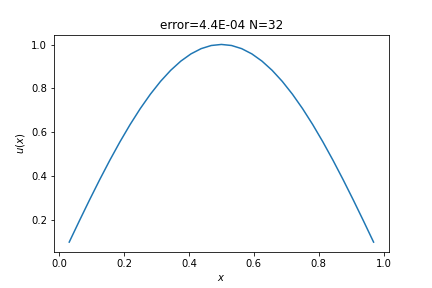
\includegraphics[scale=0.33]{hw_6_q_5_N_32.png}
        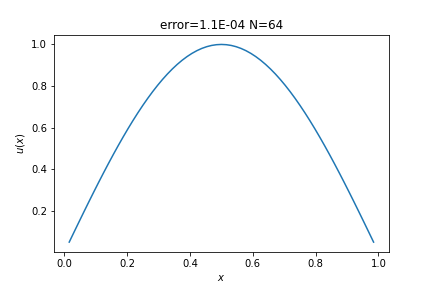
\includegraphics[scale=0.33]{hw_6_q_5_N_64.png}
        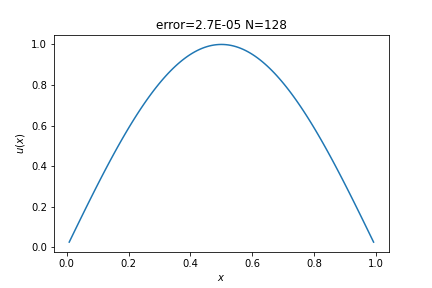
\includegraphics[scale=0.33]{hw_6_q_5_N_128.png}
        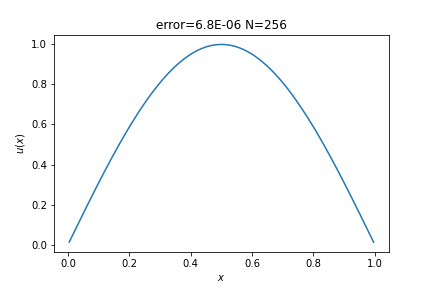
\includegraphics[scale=0.33]{hw_6_q_5_N_256.png}
        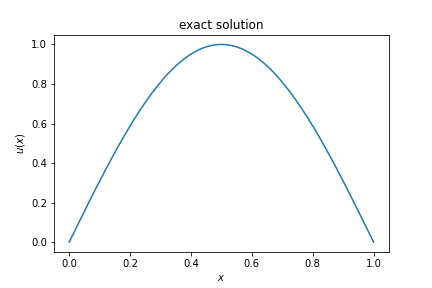
\includegraphics[scale=0.33]{exact_solution_hw_6_q_5.png}
        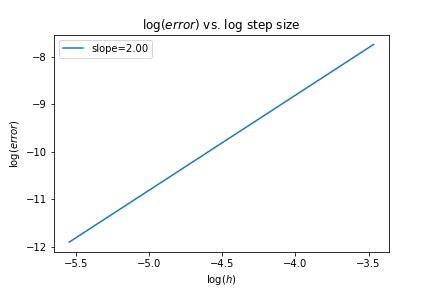
\includegraphics[scale=0.33]{q_5_error_vs_step_size.png}
    \end{figure}
\end{enumerate}
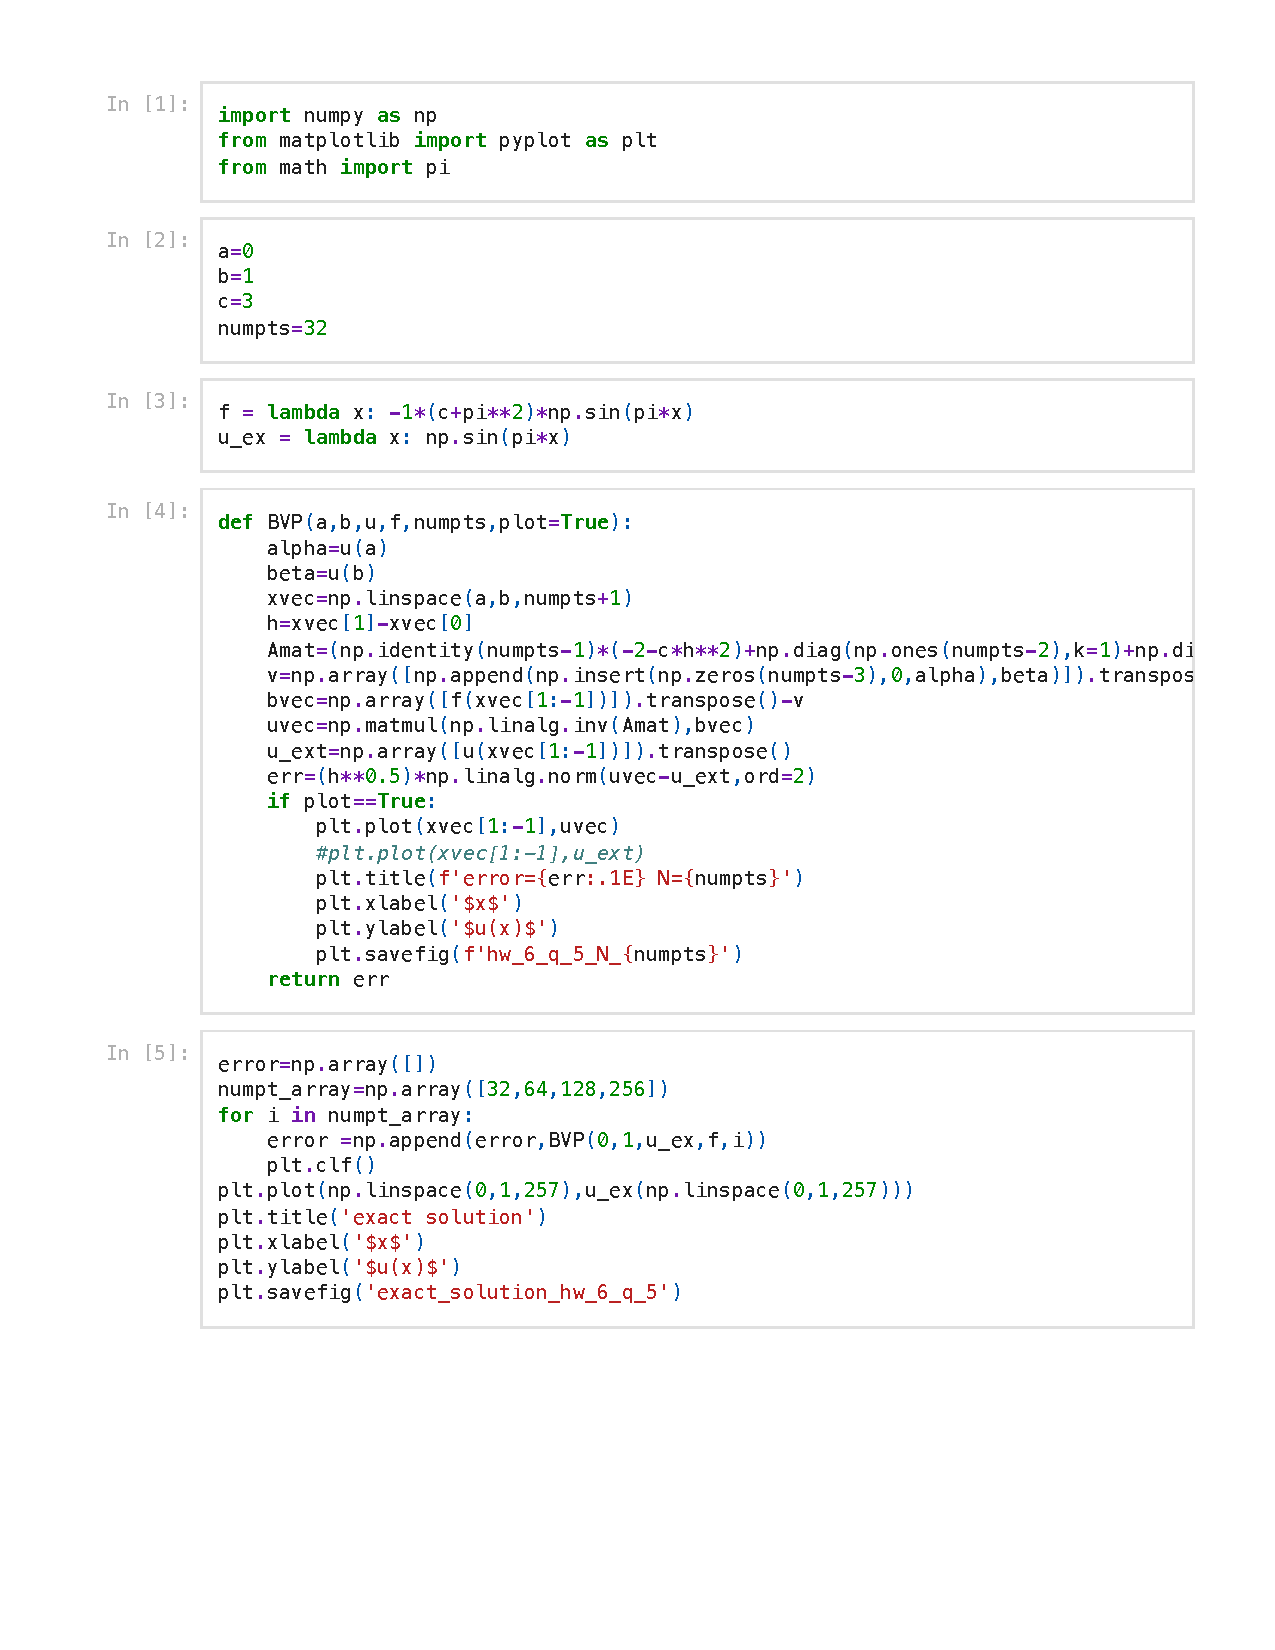
\includepdf[pages=-]{BVP_151b_2.pdf}
\end{document}